%%%%%%%%%%%%%%%%%%%%%%%%%%%%%%%%%%%%%%%%%%%%%%%%%%%%%%%%%%%%%%%%%%%%%%%%%%%%%%
%  IEEE Conference paper (IEEEtran, conference option)
%  Fast PUF-Based Authentication for UAV Swarms
%%%%%%%%%%%%%%%%%%%%%%%%%%%%%%%%%%%%%%%%%%%%%%%%%%%%%%%%%%%%%%%%%%%%%%%%%%%%%%
\documentclass[conference]{IEEEtran}
\IEEEoverridecommandlockouts

\usepackage{cite}
\usepackage{amsmath,amssymb,amsfonts}
\usepackage{amsthm}
\usepackage{bm}
\usepackage{algorithmic}
\usepackage{graphicx}
\usepackage{textcomp}
\usepackage{xcolor}
\usepackage{booktabs}
\usepackage{multirow}
\usepackage{array}
\usepackage{url}
\usepackage{balance}
\usepackage{float}
\usepackage{tikz}
\usetikzlibrary{arrows.meta,positioning,calc}
\usepackage{pgfplots}
\pgfplotsset{compat=1.18}

\def\BibTeX{{\rm B\kern-.05em{\sc i\kern-.025em b}\kern-.08em
    T\kern-.1667em\lower.7ex\hbox{E}\kern-.125emX}}

\newtheorem{theorem}{Theorem}
\newtheorem{lemma}[theorem]{Lemma}
\newtheorem{corollary}[theorem]{Corollary}

\begin{document}

\title{Fast PUF-Based Authentication for UAV Swarms\\
with GS-Free Peer Handshakes and Forward Secrecy}

\author{\IEEEauthorblockN{Md Ziyad Hussain}
\IEEEauthorblockA{\textit{Dept.\ of Computer Science and Engineering} \\
\textit{Indian Institute of Information Technology Guwahati}\\
Bongora, Assam 781015, India \\
ziyad.hussain23b@iiitg.ac.in}
\and
\IEEEauthorblockN{Rakesh Matam}
\IEEEauthorblockA{\textit{Dept.\ of Computer Science and Engineering} \\
\textit{Indian Institute of Information Technology Guwahati}\\
Bongora, Assam 781015, India \\
rakesh@iiitg.ac.in}
}

\maketitle

\begin{abstract}
A drone that carries a private key in flash memory stops being trustworthy the
moment somebody picks it up. This is the practical problem with running RSA or
ECC on a UAV swarm, and it is the problem a Physical Unclonable Function (PUF)
is meant to solve: the key is the silicon, so there is nothing in memory to
steal. We present a four-phase authentication protocol built on that idea.
Enrollment turns noisy PUF measurements into a stable per-device master key
using a BCH(255,131,18) fuzzy extractor and publishes only public helper data.
Field authentication between a UAV and its Ground Station (GS) is a four-message
handshake in which the raw PUF response never leaves the device and the UAV
refuses to answer until it has verified the GS. That handshake also hands each
UAV a set of \emph{per-pair} credentials, so any two drones can afterwards
authenticate each other with no GS round trip, and a captured drone exposes only
its own links. Every session key mixes in a mandatory authenticated ephemeral
Diffie--Hellman secret, so past traffic stays secret even if long-term material
later leaks. We implemented the protocol in C++17 on OMNeT++~6.3 (8{,}585 lines,
plus 4{,}125 lines of tests) and ran sixteen configurations, thirty
repetitions each. All 600 UAVs and all 11{,}400 peer-pair views of a twenty-drone
swarm authenticate; a UAV--GS handshake takes $0.57 \pm 0.04$~ms of compute and
$1.07$~ms of modelled network delay, and a peer handshake
$0.4167 \pm 0.0006$~ms. Executed attacks
behave as the analysis predicts, and an ablation that removes one check makes
the same attacker succeed, so the negative results are falsifiable. Running the
same handshake over a real IEEE~802.11 stack with genuine CSMA/CA contention
raises end-to-end latency to $11.9$~ms while the protocol's own compute stays at
$0.42$~ms: the increase is the channel, not the protocol. We also
report where the protocol loses: measured against real RSA-2048 and ECDSA-P256
handshakes on the same simulator, it costs $1.64$~ms against $1.77$~ms and
$0.79$~ms respectively. The gain is in properties, not in raw speed.
\end{abstract}

\begin{IEEEkeywords}
UAV swarm, physical unclonable function, fuzzy extractor, BCH code,
lightweight authentication, forward secrecy, peer-to-peer authentication.
\end{IEEEkeywords}

%=============================================================================
\section{Introduction}
%=============================================================================

UAV swarms now fly as a single operational unit: ten or twenty drones covering a
stadium, a border strip, or a collapsed building, talking constantly to a Ground
Station and to each other~\cite{securing_uav_fanet}. Before any of that traffic
can be trusted, each drone has to prove who it is, and has to check who it is
talking to. Skip that step and an attacker can slip a rogue drone into the
formation, read the telemetry, or issue flight commands~\cite{puf_uav_cross_domain}.

The obvious tools do not fit well. RSA-2048 costs about a millisecond per
signature on the hardware a drone can carry, and drags a certificate along with
every handshake~\cite{puf_lightweight_uav}. ECC-256 is much cheaper but still
keeps a private key in non-volatile memory. Pre-shared keys are fast and
collapse completely when one node is taken~\cite{puf_iot_strong_adversary}.
Blockchain schemes need seconds to reach consensus, which real-time formation
control does not have~\cite{puf_ntu}. The common thread is a long-term secret
sitting in memory on a device that can be physically recovered.

A PUF removes that secret. It maps a challenge to a response using
sub-nanometre manufacturing variation that nobody, including the
manufacturer, can reproduce, and that invasive probing
destroys~\cite{puf_overview}. An Arbiter PUF costs roughly 1{,}200 gate
equivalents. The catch is that a PUF is noisy, so its response is a
fingerprint, not a key, until a fuzzy extractor reconciles it.

\subsection{Contributions}

\begin{enumerate}
\item \textbf{A stable key with nothing stored.} Enrollment distils a per-device
master key $\text{mk}_i$ from the PUF and publishes only helper data. The drone
regenerates $\text{mk}_i$ on demand and stores no secret at all
(Section~\ref{sec:p1}).

\item \textbf{The response stays on the device.} Every handshake message carries
a MAC keyed under $\text{mk}_i$, and the UAV verifies the GS before it replies.
A forged GS therefore gets silence, not a challenge--response pair to train a
model on (Section~\ref{sec:p2}, Corollary~\ref{cor:oracle}).

\item \textbf{Peer authentication without the GS.} Phase~2 delivers per-pair
credentials under authenticated encryption, so two drones authenticate each
other directly. Capturing one node exposes only its own $N-1$ links
(Section~\ref{sec:p3}).

\item \textbf{Forward secrecy that cannot be skipped.} There is no derivation
path that omits the ephemeral Diffie--Hellman secret (Section~\ref{sec:p4}).

\item \textbf{Measured, not asserted.} A full OMNeT++ implementation, seventeen
configurations, thirty repetitions each, with per-message timing, executed
attacks against a negative control, and same-platform RSA and ECDSA baselines
including the cases where this protocol is slower
(Section~\ref{sec:eval}).
\end{enumerate}

%=============================================================================
\section{Background and Related Work}
\label{sec:related}
%=============================================================================

\subsection{PUFs and fuzzy extractors}

A PUF computes $R = \mathrm{PUF}(C)$ from physical variation. Two chips answer
the same challenge with about 50\% Hamming distance between them; one chip
answers its own challenge with a few percent of drift across temperature,
voltage, and age. That drift, typically 3\% to 10\%, is why a raw response
cannot be a key.

A fuzzy extractor $(\mathsf{Gen}, \mathsf{Rep})$ fixes this with public helper
data~\cite{dodis_fuzzy,bch_puf_extraction}. We use the code-offset construction
over a linear code $\mathsf{C}$: enrollment draws a random codeword $c$ and
publishes $s = R \oplus c$; reproduction computes $c' = R' \oplus s$ and decodes,
recovering $R$ exactly whenever $d_H(R,R') \le t$.

One point is often stated too strongly. The sketch $s$ does not perfectly hide
$R$. It pins $R$ to a coset of $\mathsf{C}$ and therefore discloses up to $n-k$
bits. The correct statement is about residual min-entropy, which we make precise
in Lemma~\ref{lem:helper} and then use to size the enrollment.

We instantiate the code as BCH(255,131,18) over $\mathrm{GF}(2^8)$: $n=255$,
$k=131$, $t=18$, $d=37$, and $n-k=124$ parity bits. At a 3\% error rate a
255-bit block is expected to flip $7.65$ bits, comfortably inside the correction
radius.

\subsection{Hash choice}

The protocol needs a 160-bit hash and nothing more exotic. We provide two
instantiations behind one interface: SHA3-256 truncated to 160
bits~\cite{sha3_standard} for software, and SPONGENT-160/160/16 for
hardware, where a few thousand gate equivalents matter more than software
throughput~\cite{spongent_original}. Switching between them changes no
protocol structure.

\subsection{Where this work sits}

Early PUF schemes authenticate one device to one
server~\cite{puf_lightweight_uav,puf_iot_strong_adversary,arbiter_puf_iot}, which
establishes the pattern but says nothing about swarm coordination. Peer
authentication has been studied with symmetric
credentials~\cite{peer2peer_auth} and across
domains~\cite{puf_uav_cross_domain,puf_6g_uav}, but usually roots peer trust in
a single shared secret, so one capture endangers the whole mesh. Table~\ref{tab:related}
places our design against representative alternatives.

\begin{table}[H]
\centering
\caption{Feature comparison against representative schemes}
\label{tab:related}
\scriptsize
\setlength{\tabcolsep}{2.6pt}
\begin{tabular}{@{}lcccccc@{}}
\toprule
\textbf{Scheme} & \textbf{PUF} & \textbf{Peer} & \textbf{No stored} &
\textbf{Fwd} & \textbf{Err} & \textbf{Formal} \\
 & & \textbf{auth} & \textbf{key} & \textbf{sec} & \textbf{corr} & \textbf{proof} \\
\midrule
RSA-2048 PKI                       & no  & yes  & no  & opt. & n/a    & partial \\
ECC-256 PKI                        & no  & yes  & no  & opt. & n/a    & partial \\
PSK (AES-GCM)                      & no  & yes  & no  & no   & n/a    & partial \\
Gope~\cite{puf_lightweight_uav}    & yes & no   & yes & no   & simple & informal \\
Li~\cite{puf_uav_cross_domain}     & yes & part.& yes & no   & BCH    & informal \\
Khan~\cite{puf_6g_uav}             & yes & no   & yes & yes  & BCH    & informal \\
Bera~\cite{peer2peer_auth}         & no  & yes  & no  & no   & n/a    & informal \\
\textbf{This work}                 & \textbf{yes} & \textbf{yes} & \textbf{yes}
                                   & \textbf{yes} & \textbf{BCH} & \textbf{games+symb.} \\
\bottomrule
\end{tabular}
\end{table}

%=============================================================================
\section{Protocol Design}
\label{sec:protocol}
%=============================================================================

\subsection{Threat model and notation}

We assume a Dolev--Yao adversary~\cite{dolev_yao} with physical reach. It may
eavesdrop, modify, replay, delay, or drop any message; it may pose as the GS and
send chosen challenges; it may capture UAVs and dump their non-volatile memory,
but it cannot clone PUF hardware, since probing destroys it. It is bounded to
probabilistic polynomial time, so it cannot invert the hash, forge a MAC or an
authenticated ciphertext, or solve computational Diffie--Hellman except with
negligible probability. Standard side-channel countermeasures are assumed.

Notation follows Table~\ref{tab:notation}. Figure~\ref{fig:overview} shows how
the phases connect.

\begin{table}[H]
\centering
\caption{Notation}
\label{tab:notation}
\footnotesize
\begin{tabular}{@{}ll@{}}
\toprule
\textbf{Symbol} & \textbf{Meaning} \\
\midrule
$\text{ID}_i,\ \text{TID}_i$ & permanent and rotating temporary identity \\
$\bm{C}_i$ & enrollment challenge block, $L$ sub-challenges \\
$R,\ R'$ & enrollment response; noisy field response \\
$P_i = (s_i, \text{seed}_i)$ & public helper data \\
$\text{mk}_i$ & per-device master key, never stored on the UAV \\
$\text{mk}_{\text{GS}}$ & GS-only key that seeds all pair credentials \\
$\text{Cred}_{ij}$ & credential shared by exactly $\text{UAV}_i,\text{UAV}_j$ \\
$K^{i}_{\text{auth}}$ & $= \mathsf{KDF}(\text{mk}_i;\ \texttt{p2-auth})$ \\
$K^{ij}_{\text{auth}}$ & $= \mathsf{KDF}(\text{Cred}_{ij};\ \texttt{peer-auth})$ \\
$h(\cdot)$ & 160-bit hash (SHA3-256$|_{160}$ or SPONGENT-160) \\
$\mathsf{MAC}_K,\ \mathsf{AE},\ \mathsf{KDF}$ & keyed MAC, AEAD, key-derivation function \\
$g^{a}, g^{ab}$ & ephemeral public share; DH secret \\
$N_x, n_x,\ T_x$ & 128-bit nonces; timestamp \\
$\mathcal{T}$ & handshake transcript \\
\bottomrule
\end{tabular}
\end{table}

\begin{figure}[H]
\centering
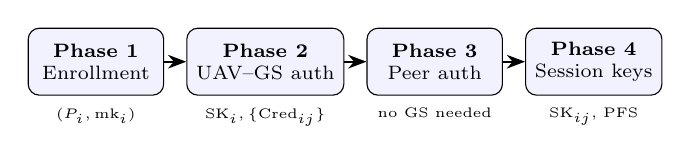
\begin{tikzpicture}[
  box/.style={draw,rounded corners,align=center,minimum height=0.85cm,
              minimum width=1.72cm,font=\scriptsize,fill=blue!5},
  >=Stealth,node distance=0.28cm]
\node[box] (p1) {\textbf{Phase 1}\\Enrollment};
\node[box,right=of p1] (p2) {\textbf{Phase 2}\\UAV--GS auth};
\node[box,right=of p2] (p3) {\textbf{Phase 3}\\Peer auth};
\node[box,right=of p3] (p4) {\textbf{Phase 4}\\Session keys};
\draw[->,thick] (p1)--(p2); \draw[->,thick] (p2)--(p3); \draw[->,thick] (p3)--(p4);
\node[font=\tiny,below=1pt of p1] {$(P_i,\text{mk}_i)$};
\node[font=\tiny,below=1pt of p2] {$\text{SK}_i,\{\text{Cred}_{ij}\}$};
\node[font=\tiny,below=1pt of p3] {no GS needed};
\node[font=\tiny,below=1pt of p4] {$\text{SK}_{ij}$, PFS};
\end{tikzpicture}
\caption{The four phases and what each produces. Phase~1 runs once in a secure
facility; the rest run in the field.}
\label{fig:overview}
\end{figure}

\subsection{Phase 1: enrollment}
\label{sec:p1}

Enrollment happens once per drone, over a trusted channel, before deployment.
The GS draws $L$ random 128-bit challenges and collects
$R = (\mathrm{PUF}_i(C_i^{(1)}), \dots, \mathrm{PUF}_i(C_i^{(L)}))$, then runs
$\mathsf{Gen}$:
\begin{align}
c &= \mathsf{C}.\mathsf{Encode}(r),\quad r \xleftarrow{\$} \{0,1\}^k, &
s &= R \oplus c, \\
\text{mk}_i &= \mathsf{KDF}\big(\mathsf{Ext}_{\text{seed}}(R);\ \texttt{root}\big), &
P_i &= (s, \text{seed}).
\end{align}
The block count $L$ is chosen so that entropy left over after the sketch leak
still covers the key:
\begin{equation}
\textstyle\sum_{b=1}^{L}\big(m_b - (n-k)\big) \;\ge\; \ell + 2\log_2(1/\varepsilon).
\label{eq:budget}
\end{equation}
The GS also fixes identities and pair credentials:
\begin{equation}
\text{Cred}_{ij} = \mathsf{KDF}\big(\text{mk}_{\text{GS}};\
  \texttt{pair-cred} \| \min(i,j) \| \max(i,j)\big).
\end{equation}
Afterwards the GS stores $\{\text{ID}_i, \text{TID}_i, \bm{C}_i, P_i, \text{mk}_i\}$
and the single $\text{mk}_{\text{GS}}$ in tamper-resistant memory. The drone
stores $\{\text{TID}_i, \bm{C}_i, P_i\}$, all of which are public. This is the
whole point: capture the drone and you get nothing, because $\text{mk}_i$ only
exists while it is being used.

\subsection{Phase 2: UAV to Ground Station}
\label{sec:p2}

Phase~2 (Fig.~\ref{fig:phase2}) is a four-message exchange that authenticates
both sides, sets up a forward-secret $\text{SK}_i$, and delivers the drone's
peer credentials. Both parties key their MACs with
$K^{i}_{\text{auth}} = \mathsf{KDF}(\text{mk}_i; \texttt{p2-auth})$: the GS from
its database, the drone from its PUF.

\begin{figure}[H]
\centering
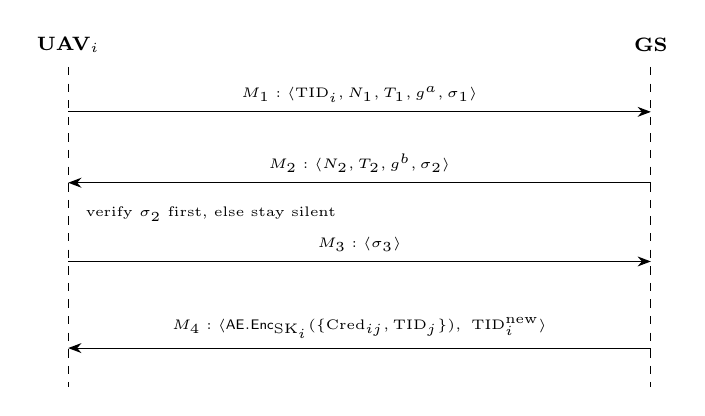
\begin{tikzpicture}[>=Stealth,font=\scriptsize]
  \node at (0,0) {\textbf{UAV$_i$}};
  \node at (7.4,0) {\textbf{GS}};
  \draw[dashed] (0,-0.28)--(0,-4.35);
  \draw[dashed] (7.4,-0.28)--(7.4,-4.35);
  \draw[->] (0,-0.85)--node[above,font=\tiny]{$M_1:\langle \text{TID}_i, N_1, T_1, g^{a}, \sigma_1\rangle$}(7.4,-0.85);
  \draw[->] (7.4,-1.75)--node[above,font=\tiny]{$M_2:\langle N_2, T_2, g^{b}, \sigma_2\rangle$}(0,-1.75);
  \node[font=\tiny,align=left,anchor=west] at (0.1,-2.15) {verify $\sigma_2$ first, else stay silent};
  \draw[->] (0,-2.75)--node[above,font=\tiny]{$M_3:\langle \sigma_3\rangle$}(7.4,-2.75);
  \draw[->] (7.4,-3.85)--node[above,font=\tiny]{$M_4:\langle \mathsf{AE}.\mathsf{Enc}_{\text{SK}_i}(\{\text{Cred}_{ij},\text{TID}_j\}),\ \text{TID}_i^{\text{new}}\rangle$}(0,-3.85);
\end{tikzpicture}
\caption{Phase~2. The drone will not answer $M_2$ until the GS authenticator
checks out, and credentials only ship after both sides are authenticated.}
\label{fig:phase2}
\end{figure}

\textbf{$M_1$.} The drone regenerates $\text{mk}_i$, picks $N_1$ and an
ephemeral scalar $a$, and sends
\begin{align}
\sigma_1 &= \mathsf{MAC}_{K^{i}_{\text{auth}}}\big(\texttt{m1} \| \text{TID}_i \| N_1 \| T_1 \| g^{a}\big),\\
M_1 &= \langle \text{TID}_i, N_1, T_1, g^{a}, \sigma_1\rangle.
\end{align}
Only a party holding $\text{mk}_i$, meaning the real drone through its PUF or
the GS through its database, can produce $\sigma_1$. The type tag \texttt{m1}
stops a token from one step being replayed as another.

\textbf{$M_2$.} The GS checks the timestamp and nonce for freshness, verifies
$\sigma_1$, and replies with its own nonce and share under
\begin{equation}
\sigma_2 = \mathsf{MAC}_{K^{i}_{\text{auth}}}\big(\texttt{m2} \| \text{TID}_i \| N_1 \| N_2 \| T_2 \| g^{a} \| g^{b}\big).
\end{equation}
Every field inside is public; the key is not, so a forged $\sigma_2$ is a MAC
forgery.

\textbf{$M_3$.} The drone verifies $\sigma_2$ \emph{before it does anything
else}, and aborts silently if the check fails. This one rule is what stops a
fake GS from using the drone as a read-out oracle. If it passes, the drone
returns $\sigma_3 = \mathsf{MAC}_{K^{i}_{\text{auth}}}(\texttt{m3} \| \mathcal{T})$
over the transcript. The PUF response itself was consumed inside $\mathsf{Rep}$
and never touches the wire.

\textbf{$M_4$.} Both sides now derive
\begin{equation}
\text{SK}_i = \mathsf{KDF}\big(\text{mk}_i \| g^{ab} \| \mathcal{T};\ \texttt{p2-sess}\big),
\label{eq:sk2}
\end{equation}
and the GS ships the credential package and a fresh identity:
\begin{align}
\text{CredPkg} &= \mathsf{AE}.\mathsf{Enc}_{\text{SK}_i}\big(\{(\text{Cred}_{ij}, \text{TID}_j)\}_{j \ne i}\big),\\
\text{TID}_i^{\text{new}} &= h(\text{TID}_i \| \text{mk}_i \| N_1 \| N_2).
\end{align}

\subsection{Phase 3: drone to drone}
\label{sec:p3}

Two drones that both completed Phase~2 share $\text{Cred}_{ij}$ and can
authenticate with no GS involvement, which matters when the command link is
down. They key on $K^{ij}_{\text{auth}} = \mathsf{KDF}(\text{Cred}_{ij}; \texttt{peer-auth})$
and exchange three messages:
\begin{align}
P_1 &= \langle n_i, T, g^{a'}, \tau_1\rangle, &
\tau_1 &= \mathsf{MAC}(\texttt{p1} \| i \| j \| n_i \| T \| g^{a'}),\\
P_2 &= \langle n_j, g^{b'}, \tau_2\rangle, &
\tau_2 &= \mathsf{MAC}(\texttt{p2} \| i \| j \| n_i \| n_j \| g^{a'} \| g^{b'}),\\
P_3 &= \langle \tau_3\rangle, &
\tau_3 &= \mathsf{MAC}(\texttt{p3} \| \mathcal{T}).
\end{align}
A third party holding some other pair's credential learns nothing about
$\text{Cred}_{ij}$, and the three distinct type tags rule out reflection. A
full mesh over $N$ drones is $N(N-1)/2$ independent exchanges, all of which can
run in parallel.

\subsection{Phase 4: session keys}
\label{sec:p4}

Both handshakes end the same way. Writing $k_{\text{lt}}$ for $\text{mk}_i$ or
$\text{Cred}_{ij}$,
\begin{equation}
\text{SK} = \mathsf{KDF}\big(k_{\text{lt}} \| g^{xy} \| \mathcal{T};\ \ell\big).
\label{eq:sk}
\end{equation}
Two independent secrets feed every key. The long-term one ties the session to
the PUF or to the pair; the ephemeral one, whose public shares were already
covered by the handshake MACs, is what gives forward secrecy once the scalars
are erased. There is no code path that omits $g^{xy}$, so a session either gets
a forward-secret key or it fails.

%=============================================================================
\section{Security Analysis}
\label{sec:security}
%=============================================================================

We assume: $h$ is pre-image, second-pre-image and collision resistant and is
modelled as a random oracle; $\mathsf{MAC}$ is EUF-CMA; $\mathsf{AE}$ is IND-CCA
and INT-CTXT; PUF responses to fresh challenges are unpredictable without the
device, and probing destroys it; gap-CDH is hard in $\mathbb{G}$.

\begin{lemma}[Helper-data privacy]
\label{lem:helper}
If $\widetilde{H}_\infty(R) = m$, then
$\widetilde{H}_\infty(R \mid P) \ge m - (n-k)$. Hence if the extractor output
length satisfies $\ell \le m - (n-k) - 2\log_2(1/\varepsilon)$, then
$\text{mk}$ is within statistical distance $\varepsilon$ of uniform given $P$.
\end{lemma}

\begin{IEEEproof}
Given the internal randomness $r$, the sketch $s = R \oplus c$ pins $R$ to a
coset of the $[n,k]$ code, which fixes at most $n-k$ syndrome bits. The chain
rule for average min-entropy gives the bound, and the seed is independent of
$R$. Applying the strong-extractor property to the residual source yields a key
within $\varepsilon$ of uniform.
\end{IEEEproof}

\begin{theorem}[Phase-2 mutual authentication]
\label{thm:mutual}
After a successful Phase~2 run, $\text{UAV}_i$ and the GS have authenticated one
another and agree on $\mathcal{T}$, except with negligible probability.
\end{theorem}

\begin{IEEEproof}
Both directions rest on $K^{i}_{\text{auth}}$, unknown to any adversary lacking
either the PUF or the GS database (Lemma~\ref{lem:helper} plus PUF
unpredictability). The GS accepts only if $\sigma_1$ and later $\sigma_3$
verify; producing a fresh valid tag without the key is an EUF-CMA forgery. The
drone accepts only if $\sigma_2$ verifies, and the same argument applies. A
nonce collision enabling transcript reuse has probability at most $q^2/2^{128}$
over $q$ sessions. Absent forgery and collision, both accepting parties hold
identical $M_1$ and $M_2$ fields, so they agree on $\mathcal{T}$.
\end{IEEEproof}

\begin{corollary}[No read-out oracle]
\label{cor:oracle}
An adversary impersonating the GS obtains no PUF response and therefore cannot
harvest challenge--response pairs for modelling.
\end{corollary}

\begin{IEEEproof}
By the verify-before-respond rule the drone emits $M_3$ only after $\sigma_2$
verifies, which by Theorem~\ref{thm:mutual} requires a forgery. On failure it
sends nothing. On success the only value transmitted is $\sigma_3$, a MAC over
public transcript fields; the response was consumed inside $\mathsf{Rep}$.
\end{IEEEproof}

\begin{theorem}[Replay and MITM resistance]
\label{thm:replay}
Phases~2 and~3 resist replay and active man-in-the-middle attacks.
\end{theorem}

\begin{IEEEproof}
Each message carries a fresh 128-bit nonce and a timestamp checked against a
window, so a verbatim replay reuses a stale value and is rejected. Each MAC
binds a per-message type tag, so a token cannot be accepted at another step.
From the second message onward each MAC binds the partner's nonce and ephemeral
share, so cross-session reuse produces a mismatch. Altering any covered field
invalidates its tag, and forging one requires the key. Combined with the
agreement of Theorem~\ref{thm:mutual}, an interposed adversary cannot remain
undetected.
\end{IEEEproof}

\begin{theorem}[Peer authentication]
\label{thm:peer}
After a successful Phase~3 run, $\text{UAV}_i$ and $\text{UAV}_j$ have
authenticated one another without GS involvement, and no per-pair secret is
exposed in transit.
\end{theorem}

\begin{IEEEproof}
$\text{Cred}_{ij}$ reaches each endpoint only inside
$\mathsf{AE}.\mathsf{Enc}_{\text{SK}_i}(\cdot)$. INT-CTXT prevents substitution
and IND-CCA hides the value. Given a secret $\text{Cred}_{ij}$, each of
$\tau_1,\tau_2,\tau_3$ binds both identities and both nonces, so an acceptance
forces a matching computation by the partner or an EUF-CMA forgery. Credentials
are pair-specific, so a holder of $\text{Cred}_{k\ell}$ learns nothing about
$\text{Cred}_{ij}$.
\end{IEEEproof}

\begin{theorem}[Session-key secrecy and forward secrecy]
\label{thm:pfs}
For an adversary corrupting neither endpoint, the key of Eq.~\eqref{eq:sk} is
indistinguishable from uniform. If the ephemeral scalars are erased, revealing
$\text{mk}_i$, $\text{Cred}_{ij}$, or $\text{mk}_{\text{GS}}$ after the session
closes does not compromise it.
\end{theorem}

\begin{IEEEproof}
Modelling $\mathsf{KDF}$ as a PRF, replacing it by a random function is
undetectable up to its PRF advantage. Two independent secrets feed it:
$k_{\text{lt}}$, protected by Lemma~\ref{lem:helper} and PUF unpredictability
or by Theorem~\ref{thm:peer}, and $g^{xy}$, unpredictable under gap-CDH given
only the authenticated shares. For forward secrecy, a post-session reveal gives
$k_{\text{lt}}$ but not the erased scalars, so the adversary must compute
$g^{xy}$ from the recorded shares, a gap-CDH instance. Because the exchange is
mandatory there is no non-ephemeral fallback.
\end{IEEEproof}

\begin{theorem}[Capture resistance]
\label{thm:capture}
Capturing $\text{UAV}_k$ and reading its memory does not let the adversary
impersonate any other UAV to the GS, nor any pair not involving $k$. Exposure is
bounded to $k$'s own $N-1$ links.
\end{theorem}

\begin{IEEEproof}
The captured memory holds $\{\text{TID}_k, \bm{C}_k, P_k, \{\text{Cred}_{kj}\}_j\}$
and any live session keys. The first three are public. Impersonating
$\text{UAV}_m$, $m \ne k$, needs $K^{m}_{\text{auth}}$, hence $\text{mk}_m$,
which is never stored, is not recoverable from $k$'s silicon by tamper
evidence, and is unpredictable, so this reduces to a MAC forgery. Impersonating
a pair $(m,\ell)$ with $k \notin \{m,\ell\}$ needs
$\text{Cred}_{m\ell} = \mathsf{KDF}(\text{mk}_{\text{GS}}; \cdot)$, independent
of every captured $\text{Cred}_{kj}$ because the KDF inputs differ and
$\text{mk}_{\text{GS}}$ never leaves the GS.
\end{IEEEproof}

These reductions are mirrored by a symbolic model in the Tamarin
prover~\cite{tamarin}, whose multiset-rewriting calculus handles freshness,
stateful credential issuance, and device compromise natively. Two extra rules
model compromise: one reveals a captured node's memory but neither its PUF nor
its master key, and one reveals long-term secrets after a session closes for the
forward-secrecy query. PUF noise is idealised there as a noiseless private
function, since error tolerance is a correctness property of the fuzzy
extractor rather than a symbolic one.

%=============================================================================
\section{Implementation}
\label{sec:impl}
%=============================================================================

The protocol is implemented in C++17 on OMNeT++~6.3: 8{,}585 lines in
\texttt{src/} plus 4{,}125 lines of tests. Protocol logic
(\texttt{GroundStationProtocol}, \texttt{UavProtocol}) depends only on abstract
crypto interfaces and byte strings, with no reference to the simulation kernel,
so the whole four-phase exchange can be driven over an in-memory transport and
validated independently of the network model. Because the transport-agnostic
layer is reused verbatim, the same protocol objects run over both the idealised
medium and a real INET 802.11 stack; only the transport differs, which is what
makes the two tracks directly comparable. The two tracks also differ in clock
model, and the results say so: on the idealised medium compute is host
wall-clock while network is simulated and the two never meet, so their sum is the
realistic total; on INET and the signature baselines everything runs on the
simulation clock, so measured wall time is the total and network is derived as
$\text{wall}-\text{compute}$.

\subsection{Canonical encoding}

One encoder produces the wire image, the MAC input, and the byte count that
drives link delay, so reported overhead cannot drift from what is actually
sent. Each field is a type tag, a two-byte length, and a value, under a header
carrying protocol version, suite id, and message type, with tags emitted in
strictly ascending order:
\begin{align}
\mathsf{field}(t,v) &= \mathsf{u8}(t) \| \mathsf{u16}(|v|) \| v,\\
\mathsf{enc} &= \mathsf{u8}(\text{ver}) \| \mathsf{u8}(\text{suite}) \| \mathsf{u8}(\text{type}) \notag\\
             &\quad \| \mathsf{u16}(k) \| \mathsf{field}(t_1,v_1)\cdots
\end{align}
The encoding is therefore injective and canonical, which is exactly what the
unforgeability argument needs of its MAC inputs. Duplicate or out-of-order tags
are rejected rather than tolerated.

\subsection{Two suites}

\begin{table}[H]
\centering
\caption{The two cryptographic profiles}
\label{tab:suites}
\footnotesize
\setlength{\tabcolsep}{3.5pt}
\begin{tabular}{@{}lll@{}}
\toprule
\textbf{Component} & \textbf{\texttt{sha3}} & \textbf{\texttt{spongent}} \\
\midrule
Hash $h$        & SHA3-256 trunc.\ 160 & SPONGENT-160/160/16 \\
MAC             & HMAC-SHA3-256, 128-bit tag & prefix keyed sponge \\
KDF             & HKDF & one-pass sponge \\
AEAD            & ChaCha20-Poly1305 & Ascon-128a v1.2 \\
Key exchange    & X25519 & X25519 \\
Hash/MAC level  & 128-bit & 80-bit ($c=160$) \\
Provenance      & OpenSSL 3.5 & vendored \\
\bottomrule
\end{tabular}
\end{table}

Table~\ref{tab:suites} lists both. Three points need saying plainly. First,
HMAC is not applicable to the sponge profile: HMAC needs $|K| \le B$ for block
size $B$, and SPONGENT-160/160/16 has a 16-bit rate, so the block is two bytes.
The construction is simply undefined there, and an ad-hoc substitute would have
no proof behind it. We use the standard prefix keyed sponge underlying
KMAC~\cite{sha3_standard} instead, which is sound for a sponge with non-zero
capacity because such a sponge is not length-extendable. Second, at $c=160$ the
keyed-sponge bound gives roughly 80 bits, deliberately asymmetric with the
128-bit AEAD and key exchange; we present it as a constrained-hardware profile
at that level and not as a 128-bit one. Third, every derived key carries a
unique label (\texttt{p2-auth}, \texttt{p2-sess}, \texttt{pair-cred},
\texttt{peer-auth}, \texttt{peer-sess}, \texttt{tid-rotate}) and distinct domain
bytes separate hash, MAC, and KDF modes even where they share a permutation.

All protocol randomness comes from a deterministic generator seeded from the
simulator's stream, including ephemeral X25519 scalars, so an entire run is
reproducible from its seed.

\subsection{Code and fuzzy extractor}

The BCH generator polynomial is the product of the minimal polynomials of
$\alpha^1,\dots,\alpha^{2t}$ over the complete conjugate closure of each root.
For $t=18$ over $\mathrm{GF}(2^8)$ that closure has 124 roots, so $\deg g = 124$
and $k = 131$. Both facts are asserted at construction. This matters: taking the
parity length as $mt = 144$ instead would give $k = 111$ and silently leave the
tail of every 128-bit response uncovered. Decoding runs syndromes,
Berlekamp--Massey, and a Chien search, then verifies that the corrected word has
all-zero syndromes. Failure is reported as failure, never as a silent pass-through.

Because the sketch discloses up to $n-k = 124$ bits per block, blocks must be
longer than the leak to be worth anything, which is why blocks are 255 bits and
not the 128 bits of a native challenge--response pair. The budget of
Eq.~\eqref{eq:budget} is enforced at construction and raises an error when
unmet. With entropy rate $\rho = 0.95$, $\ell = 256$ and $\varepsilon = 2^{-64}$,
each block contributes $118.25$ bits and $L=4$ gives $473 \ge 384$. Reproduction
fails closed: if any block fails to decode, no key material is returned.

\subsection{PUF models and verification}

Three PUF models are provided and every result states which it used. The
\emph{ideal} model realises the strong-PUF abstraction as a keyed PRF. The
\emph{arbiter} model implements the additive-delay formulation over 128 stages
with per-device Gaussian weights, adding noise to the accumulated delay
difference rather than flipping output bits:
\begin{equation}
\Delta' = \textstyle\sum_i w_i \phi_i + \mathcal{N}(0,\sigma), \qquad r = \mathbb{1}[\Delta' > 0].
\end{equation}
Bits whose delay difference sits near zero therefore flip far more often than
the rest, which is how real silicon behaves; the measured variance of per-bit
flip rates is about $98\times$ that of a uniform bit-flip channel, a structural
property a per-bit model cannot show. A third model XORs $k$ arbiter chains.

Both models return a whole response from one keyed stream rather than one
evaluation per bit: the ideal model is the concatenation of successive 256-bit
blocks of $\mathsf{HMAC}_{\text{SHA3-256}}(k_{\text{dev}}, \ell \| C \| n)$,
truncated to the response length, so four calls cover the 1020-bit response the
default profile needs, and the arbiter model draws all of its sub-challenges from
one analogous $\mathsf{SHA3\text{-}256}$ stream. This is a simulation-cost choice
with no cryptographic effect --- the object is the same keyed PRF per device with
independent uniform output bits --- but evaluating each bit separately cost two
hash calls per bit and made the simulated PUF the slowest part of a protocol
whose real device answers in nanoseconds. Noise is applied as a 16-bit threshold
on two PRNG bytes per bit, an exact Bernoulli($p$) channel to 16-bit precision,
with the same two bytes drawn whatever $p$ is, so a run stays reproducible when
the noise setting changes. Over 24 devices and 276 pairs, inter-device Hamming
distance is $0.5019$ (arbiter) and $0.5026$ (ideal), and calibrated bit-error
rates track their targets within 0.2 percentage points from 1\% to 10\%.

Each primitive is checked against published vectors where they exist:
FIPS~202/CAVP for SHA3-256, NIST intermediate values for HMAC-SHA3-256, RFC~5869
A.1 to A.3 for HKDF, RFC~8439 \S2.8.2 for ChaCha20-Poly1305, RFC~7748 \S6.1 for
X25519 with low-order points rejected, and all 1{,}089 vectors of the official
Ascon-128a known-answer-test file. SPONGENT-160 has no official KAT file, so we
check byte-exact agreement with the designers' reference implementation and the
published digest, and claim nothing more. BCH is checked for $\deg g = 124$,
$g(x) \mid x^{255}+1$, exact recovery in all 18{,}000 trials at weights 1 to 18,
and correct failure reporting in 3{,}000 trials beyond the radius. Neither
vendored primitive has had timing or side-channel analysis; tag comparison is
constant-time and no branch depends on secret data, but nothing stronger is
claimed.

\subsection{Simulation model}

$N$ UAVs sit around a $500 \times 300$~m field with the GS at the centre. Link
delay is propagation from node coordinates, plus serialisation at the configured
6~Mbps, plus a fixed processing delay, plus half-normal jitter, each reported
separately per message. This primary model does not simulate MAC-layer
contention, so its network delay is a lower bound; Section~\ref{sec:inet}
brackets it from above with a real IEEE~802.11 stack.

%=============================================================================
\section{Evaluation}
\label{sec:eval}
%=============================================================================

All runs are on an AMD Ryzen 5 5625U with OpenSSL~3.5.5 and OMNeT++~6.3. Every
configuration changes exactly one variable against the reference
\texttt{StadiumSHA3}, so a difference in outcome can be attributed to that
variable.

\subsection{Methodology}

Each configuration runs thirty independent repetitions with distinct seed sets
(five for attacks). The unit of replication is the \emph{run}, not the
individual record: observations inside one run share a pseudorandom stream and a
scheduling epoch, so they are correlated. Confidence intervals are therefore
two-stage, a per-run mean followed by a $t$-interval across run means with $R-1$
degrees of freedom. Pooling all records instead would inflate the degrees of
freedom from $R-1$ to $NR-1$ and understate every interval by roughly
$\sqrt{N}$. Proportions carry Wilson score intervals, which behave correctly
near 0 and 1.

Compute times are host wall-clock; network delays are simulated. These are
different clocks, reported separately and never silently summed. Where a single
realistic figure is needed we use Compute $+$ Network and say so, except on the
real-802.11 track, where everything runs on one clock and measured end-to-end
wall time is itself the total (network there being derived as wall $-$ compute).

\subsection{Functional correctness}

\begin{table}[H]
\centering
\caption{Authentication outcomes, 30 repetitions per configuration}
\label{tab:functional}
\scriptsize
\setlength{\tabcolsep}{3pt}
\begin{tabular}{@{}lccccc@{}}
\toprule
\textbf{Configuration} & \textbf{Dev.} & \textbf{Auth.} & \textbf{Rate} &
\textbf{Wilson 95\%} & \textbf{Peer pairs} \\
\midrule
StadiumSHA3 ($N{=}10$)     & 300 & 300 & 1.000 & [0.987, 1.000] & 2700/2700 \\
StadiumSPONGENT ($N{=}10$) & 300 & 300 & 1.000 & [0.987, 1.000] & 2700/2700 \\
Baseline5UAV ($N{=}5$)     & 150 & 150 & 1.000 & [0.975, 1.000] & 600/600 \\
Swarm20 ($N{=}20$)         & 600 & 600 & 1.000 & [0.994, 1.000] & 11400/11400 \\
ArbiterPuf (3\% BER)       & 300 & 298 & 0.993 & [0.976, 0.998] & 2664/2690 \\
HighNoise (5\% BER)        & 300 & 247 & 0.823 & [0.776, 0.862] & 1830/2214 \\
\bottomrule
\end{tabular}
\end{table}

Table~\ref{tab:functional} separates two rates on purpose. One counts drones
that transmitted a first message; the other counts all enrolled devices. They
diverge when a drone cannot reproduce its master key, in which case it never
initiates at all, and reporting only the first would hide that failure mode
completely. With the ideal PUF every device authenticates in every
configuration, including the twenty-drone swarm where all 11{,}400 peer-pair
views complete. Under the arbiter model at 3\% two devices in three hundred fail
to regenerate; at 5\%, fifty-three do. Those are fuzzy-extractor reliability
limits, not authentication failures.

\subsection{Latency and overhead}

\begin{table}[H]
\centering
\caption{Phase-2 cost (mean $\pm$ 95\% CI, 30 runs). Compute and Network are
separate measurements on two clocks; their sum is the realistic total}
\label{tab:latency}
\scriptsize
\setlength{\tabcolsep}{2.6pt}
\begin{tabular}{@{}lccc@{}}
\toprule
\textbf{Configuration} & \textbf{Compute} &
\textbf{Network} & \textbf{Bytes} \\
 & \textbf{(ms)} & \textbf{(ms)} & \\
\midrule
StadiumSHA3     & $0.569{\pm}0.036$ & $1.074{\pm}0.002$ & 777 \\
StadiumSPONGENT & $3.456{\pm}0.102$ & $1.079{\pm}0.002$ & 781 \\
Baseline5UAV    & $0.458{\pm}0.003$ & $0.714{\pm}0.003$ & 507 \\
Swarm20         & $0.487{\pm}0.023$ & $1.790{\pm}0.006$ & 1315 \\
\bottomrule
\end{tabular}
\end{table}

Compute varies by nearly $6\times$ across the two profiles while network delay
is identical to four significant figures, because the link model depends only on
message size and position, neither of which the suite changes.

Phase-3 peer authentication costs $0.4166 \pm 0.0006$~ms per pair with 197~bytes
of traffic, pooled across the four configurations that vary swarm size. The
per-configuration means ($0.4171$, $0.4171$, $0.4163$, $0.4159$~ms) agree inside
their own intervals, so the pooled figure is independent of $N$: the $O(N^2)$
growth in total cost comes entirely from the pair count and not from a per-pair
cost that grows.

Phase-2 overhead grows with $N$ because the credential package in $M_4$ carries
one credential per peer: 275~B at $N=5$, 545~B at $N=10$, 1{,}085~B at $N=20$,
against a fixed 232~B for $M_1$ to $M_3$. An on-demand variant issuing
credentials per request is a straightforward extension where this matters.

\subsection{Where the time goes}

\begin{table}[H]
\centering
\caption{Phase-2 message breakdown, mean over 300 handshakes per suite}
\label{tab:msg}
\scriptsize
\setlength{\tabcolsep}{2.4pt}
\begin{tabular}{@{}llrrrr@{}}
\toprule
\textbf{Msg} & \textbf{Work done} & \textbf{\texttt{sha3}} & \textbf{\texttt{spg}} &
\textbf{Net} & \textbf{B} \\
 & & \textbf{(ms)} & \textbf{(ms)} & \textbf{(ms)} & \\
\midrule
$M_1$ & UAV: PUF $+$ \texttt{Rep} $+$ MAC & 0.3703 & 0.9323 & 0.2554 & 104 \\
      & \quad of which PUF evaluation     & 0.0421 & 0.0405 & --- & --- \\
      & \quad of which BCH decode         & 0.2452 & 0.5123 & --- & --- \\
      & GS: verify $\sigma_1$             & 0.0595 & 0.6113 & --- & --- \\
$M_2$ & UAV: verify $\sigma_2$ (the gate) & 0.0934 & 1.1953 & 0.2303 & 85 \\
$M_3$ & UAV: compute $\sigma_3$           & 0.0934 & 1.1953 & 0.1737 & 43 \\
      & GS: verify $\sigma_3$ $+$ sess.\ KDF & 0.1576 & 2.4677 & --- & --- \\
$M_4$ & GS: AEAD-seal credentials         & 0.0122 & 0.1335 & 0.8433 & 545/549 \\
\midrule
\textbf{Total} & & \textbf{0.569} & \textbf{3.456} & \textbf{1.074/1.079} & \textbf{777/781} \\
\bottomrule
\end{tabular}
\end{table}

Table~\ref{tab:msg} shows three things the summary numbers do not.

$M_1$ carries the largest single cost, and it is not the PUF. Under
\texttt{sha3}, BCH reproduction alone is $0.245$~ms, which is 66\% of $M_1$'s own
compute and 43\% of the entire handshake, while the PUF evaluation is $0.042$~ms.
The drone needs $\text{mk}_i$ to authenticate $M_1$ in the first place, so
\texttt{Rep} necessarily runs before $M_1$ is sent, not at $M_3$ where a reading
of the phase ordering might place it; that ordering is also why the PUF and error
correction both belong to $M_1$ in the measured breakdown.

Network delay is identical across suites to four significant figures, because
link delay depends only on message size and node position, neither of which the
suite changes materially. So the entire compute gap, a factor of $6.1$, belongs
to the crypto suite alone.

That gap concentrates in $M_2$ and $M_3$. Each performs one MAC with no PUF or
AEAD work beside it, so the suite difference shows almost in isolation:
\texttt{spongent}'s keyed sponge costs about $13\times$ \texttt{sha3}'s HMAC
there, consistent with the $225~\mu$s against $2.4~\mu$s per-call figures in
Table~\ref{tab:prim}. $M_1$'s gap is diluted by the shared error-correction cost,
and $M_4$ barely differs at all, since Ascon-128a is not slower than
ChaCha20-Poly1305 here.

$M_1$ is where the largest single cost sits, and it is not the PUF: BCH
reproduction is $0.245$~ms under \texttt{sha3} and $0.512$~ms under
\texttt{spongent}, roughly two-thirds and half of $M_1$'s compute, while the PUF
evaluation itself is $0.04$~ms under either suite.

Phase~3 never touches the PUF. Its three messages cost $0.0277$, $0.0286$, and
$0.0477$~ms of compute under \texttt{sha3} and $0.1724$, $0.2885$, $0.5517$~ms
under \texttt{spongent}, which is why peer authentication is roughly a fifth
of Phase-2's compute and why the suite gap there is wider with no PUF or AEAD
cost to dilute it.

\subsection{Primitive costs against public-key baselines}

\begin{table}[H]
\centering
\caption{Median per-call cost, same host and library throughout}
\label{tab:prim}
\footnotesize
\setlength{\tabcolsep}{4pt}
\begin{tabular}{@{}llrr@{}}
\toprule
\multicolumn{4}{@{}l}{\textit{This work, measured in-protocol ($\mu$s/call)}} \\
\textbf{Operation} & & \textbf{\texttt{sha3}} & \textbf{\texttt{spongent}} \\
\midrule
Hash$^{\ddagger}$    & & 0.49  & ---    \\
MAC                  & & 2.41  & 224.82 \\
MAC verify           & & 2.46  & 236.22 \\
KDF                  & & 5.51  & 132.71 \\
Extract              & & 3.42  & 291.20 \\
AEAD seal            & & 2.66  & 1.64   \\
AEAD open            & & 1.58  & 1.47   \\
X25519 keygen$^{\dagger}$  & & 36.85 & 33.87 \\
X25519 derive$^{\dagger}$  & & 71.63 & 65.05 \\
\midrule
\multicolumn{4}{@{}l}{\textit{Public-key baselines, tight-loop benchmark}} \\
\textbf{Scheme} & \textbf{Op.} & \textbf{Median} & \textbf{Mean} \\
\midrule
RSA-2048     & sign    & 530.3 & 541.7 \\
RSA-2048     & verify  & 16.9  & 17.3 \\
ECDSA P-256  & sign    & 20.4  & 21.3 \\
ECDSA P-256  & verify  & 57.2  & 57.8 \\
ECDH P-256   & derive  & 51.7  & 55.5 \\
X25519       & keygen$^{\dagger}$ & 36.1 & 42.9 \\
X25519       & derive$^{\dagger}$ & 64.1 & 64.8 \\
\bottomrule
\end{tabular}

\vspace{2pt}
\raggedright\scriptsize
$^{\dagger}$X25519 appears in both blocks because it is the one operation they
share. The same code is measured in both contexts and, on a thermally
unconstrained run, the two agree ($37$--$72~\mu$s in-protocol against
$36$--$64~\mu$s benchmarked), so either may be used; the benchmarked row is the
one compared against ECDH and ECDSA below. An earlier run reported roughly double
these values, which proved to be thermal throttling rather than a
measurement-context effect.
$^{\ddagger}$Hash is the only in-protocol row taken from the dedicated
benchmark: the protocol never calls a standalone hash at top level, so no
in-protocol call count exists for it.
\end{table}

\begin{figure}[H]
\centering
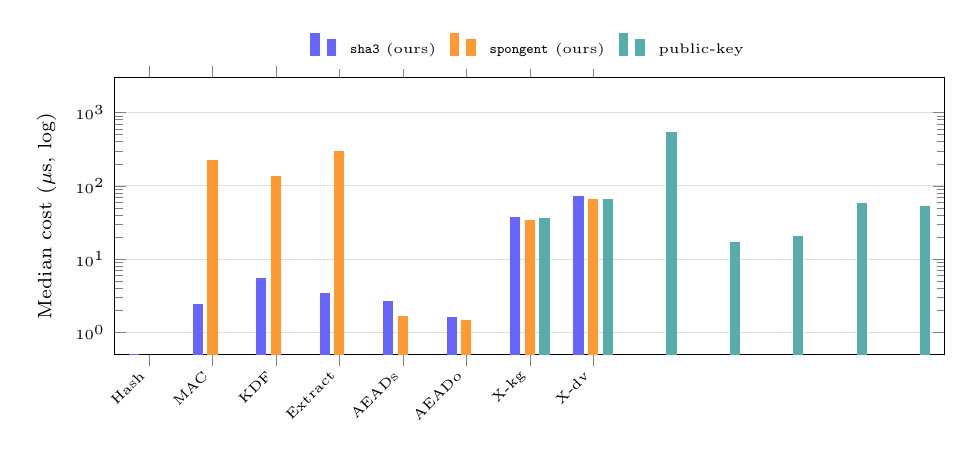
\begin{tikzpicture}
\begin{axis}[
  ybar, bar width=3.3pt, width=\linewidth, height=5.1cm,
  ymode=log, log origin=infty, ymin=0.5, ymax=3000,
  ylabel={Median cost ($\mu$s, log)}, ylabel style={font=\scriptsize},
  symbolic x coords={Hash,MAC,KDF,Extract,AEADs,AEADo,X-kg,X-dv,
    RSAs,RSAv,ECDSAs,ECDSAv,ECDHd},
  xtick=data, x tick label style={rotate=45,anchor=east,font=\tiny},
  ytick={1,10,100,1000}, yticklabel style={font=\tiny},
  enlarge x limits=0.045, ymajorgrids, grid style={gray!25},
  legend style={at={(0.5,1.03)},anchor=south,legend columns=3,font=\tiny,
                draw=none,column sep=3pt},
  ]
\addplot[fill=blue!60,draw=blue!60] coordinates
  {(Hash,0.49) (MAC,2.41) (KDF,5.51) (Extract,3.42) (AEADs,2.66) (AEADo,1.58)
   (X-kg,36.85) (X-dv,71.63)};
\addplot[fill=orange!80,draw=orange!80] coordinates
  {(MAC,224.82) (KDF,132.71) (Extract,291.20) (AEADs,1.64) (AEADo,1.47)
   (X-kg,33.87) (X-dv,65.05)};
\addplot[fill=teal!65,draw=teal!65] coordinates
  {(RSAs,530.3) (RSAv,16.9) (ECDSAs,20.4) (ECDSAv,57.2) (ECDHd,51.7)
   (X-kg,36.1) (X-dv,64.1)};
\legend{\texttt{sha3} (ours),\texttt{spongent} (ours),public-key}
\end{axis}
\end{tikzpicture}
\caption{Per-call primitive cost on one logarithmic axis (Table~\ref{tab:prim}).
No \texttt{spongent} Hash bar is drawn, matching the dash in the table.}
\label{fig:prim}
\end{figure}

Three readings follow from Table~\ref{tab:prim} and Fig.~\ref{fig:prim}.

Every \texttt{sha3} symmetric primitive beats every measured asymmetric one.
Our most expensive is KDF at $5.5~\mu$s, still several times under the cheapest
baseline shown (RSA-2048 verify, $16.9~\mu$s). This is a fair comparison
because both sides are isolated primitive calls timed the same way.

The \texttt{spongent} suite does not carry that advantage. Its MAC, KDF, and
Extract land at $133$ to $291~\mu$s, above rather than below the asymmetric
baselines ($17$ to $64~\mu$s). That is the direct cost of a
hardware-area-optimised permutation running in software, and it does not
undercut the area argument that motivates the profile in the first place.

Neither reading is a protocol-level claim. Note also that RSA-2048
\emph{verification} costs about $17~\mu$s here, so the millisecond figures
sometimes quoted for it, and any speedup multiplier derived from them, are off
by two to three orders of magnitude. And our own mandatory ephemeral exchange
(X25519 keygen $+$ derive, about $100~\mu$s under the like-for-like figure) is
comparable to an ECDH or ECDSA exchange at $52$ to $78~\mu$s, not faster. That
is what forward secrecy costs.

\subsection{Full-protocol comparison}
\label{sec:baseline}

\begin{table}[H]
\centering
\caption{Full four-message handshake, same simulator, host, and OpenSSL build
(mean $\pm$ 95\% CI, 30 runs each)}
\label{tab:base}
\scriptsize
\setlength{\tabcolsep}{2.6pt}
\begin{tabular}{@{}lcccc@{}}
\toprule
\textbf{Protocol} & \textbf{Compute} & \textbf{Network} &
\textbf{C$+$N} & \textbf{Bytes} \\
 & \textbf{(ms)} & \textbf{(ms)} & \textbf{(ms)} & \\
\midrule
RSA-2048 signed eph.\ DH   & $1.069{\pm}0.005$ & $0.699{\pm}0.002$ & 1.77 & 703 \\
ECDSA-P256 signed eph.\ DH & $0.341{\pm}0.005$ & $0.452{\pm}0.002$ & 0.79 & 333 \\
\midrule
This work (\texttt{sha3})     & $0.569{\pm}0.036$ & $1.074{\pm}0.002$ & 1.64 & 777 \\
This work (\texttt{spongent}) & $3.456{\pm}0.102$ & $1.079{\pm}0.002$ & 4.54 & 781 \\
\bottomrule
\end{tabular}
\end{table}

\begin{figure}[H]
\centering
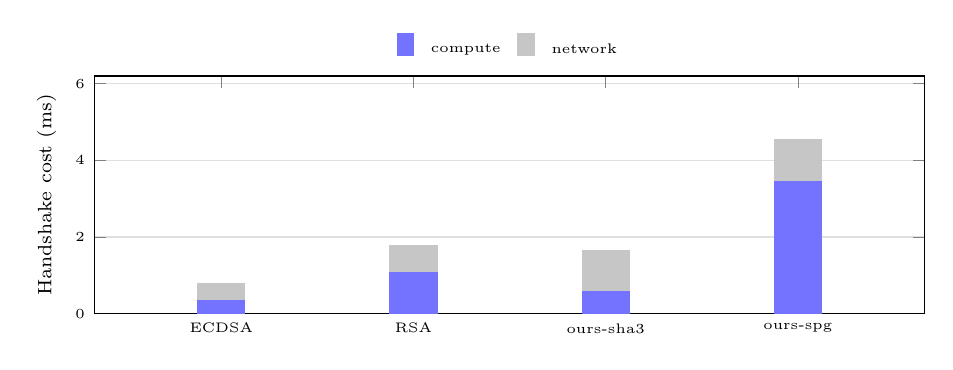
\begin{tikzpicture}
\begin{axis}[
  ybar stacked, bar width=17pt, width=\linewidth, height=4.6cm,
  ymin=0, ymax=6.2, ylabel={Handshake cost (ms)},
  ylabel style={font=\scriptsize}, yticklabel style={font=\tiny},
  symbolic x coords={ECDSA,RSA,{ours-sha3},{ours-spg}},
  xtick=data, x tick label style={font=\tiny},
  enlarge x limits=0.22, ymajorgrids, grid style={gray!25},
  legend style={at={(0.5,1.03)},anchor=south,legend columns=2,font=\tiny,
                draw=none,column sep=4pt},
  ]
\addplot[fill=blue!55,draw=blue!55] coordinates
  {(ECDSA,0.3410) (RSA,1.0685) ({ours-sha3},0.5693) ({ours-spg},3.4564)};
\addplot[fill=gray!45,draw=gray!45] coordinates
  {(ECDSA,0.4523) (RSA,0.6990) ({ours-sha3},1.0737) ({ours-spg},1.0790)};
\legend{compute,network}
\end{axis}
\end{tikzpicture}
\caption{Full-handshake cost against real signature-authenticated baselines
(Table~\ref{tab:base}). This work is slower than ECDSA and close to RSA.}
\label{fig:base}
\end{figure}

We built and ran two real baseline protocols through the same simulator, host,
OpenSSL build, and link-delay model: a signature-authenticated ephemeral X25519
exchange, once with RSA-2048 and once with ECDSA-P256 replacing our PUF-derived
MAC. Each is a genuine four-message mutual handshake $B_1$ to $B_4$ mirroring
$M_1$ to $M_4$: the initiator signs its nonce and share, the responder verifies
that signature before doing anything else, replies with its own signed nonce and
share, and both derive a session key from the completed exchange and confirm it
with a symmetric MAC. That is the same division of labour TLS~1.3 uses, so
neither baseline is a straw man. Long-term keypairs are provisioned once, out of
band, exactly as our own challenge and helper data are.

Two findings come out, and they point in different directions.

\textbf{Against RSA we now come out ahead.} $1.64$~ms against $1.77$~ms is a
narrow but genuine win, and it is not the direction a primitive-level reading
would predict. The reason is visible in the Compute column: RSA-2048 signing
costs $0.81$~ms per handshake in-protocol, consistent with the $530~\mu$s
tight-loop figure, which is more than our entire protocol compute. Charging RSA
its real signing cost is what closes the gap, not any speed advantage in our own
primitives.

\textbf{Against ECDSA we are genuinely slower.} $0.79$~ms against $1.64$~ms is a
real gap of $2.1\times$. ECDSA-P256 signing is cheap at $20~\mu$s, so an
ECDSA-authenticated handshake pays almost nothing beyond the ephemeral exchange
itself. We pay the PUF reproduction and error-correction cost on every handshake,
and in return store no long-term secret on the device at all. That is the honest
price of this threat model against a scheme whose signing key is cheap to use but
has to live somewhere a captured device can surrender it.

Overhead follows the same pattern for a different reason. RSA's 256-byte
signature, sent in both directions, drives its 703~B total. ECDSA's short
DER-encoded signature is the cheapest at 333~B, varying run to run with the
encoded length of $r$ and $s$. Our 777~B includes a per-peer credential
package that neither baseline carries, because GS-free peer authentication is a
property neither baseline has.

\subsection{Fuzzy-extractor reliability}

\begin{figure}[H]
\centering
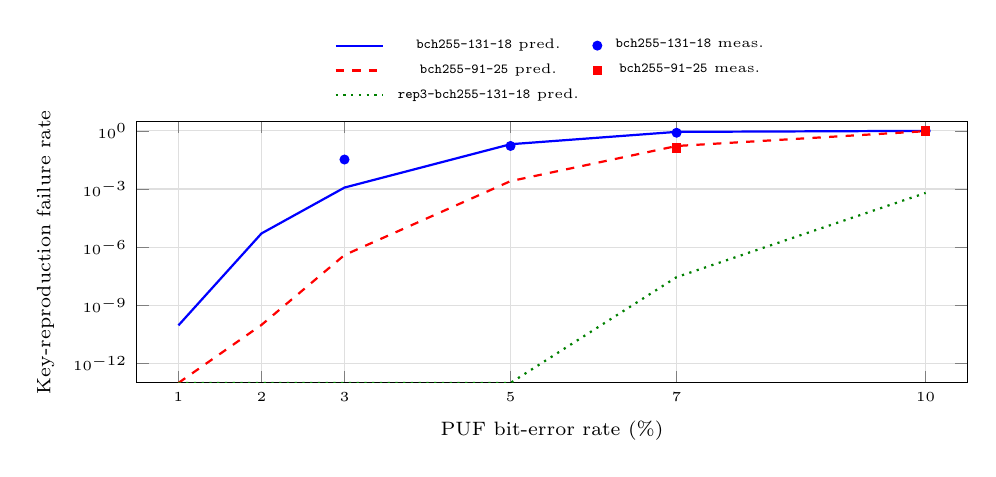
\begin{tikzpicture}
\begin{axis}[
  width=\linewidth, height=4.9cm,
  xlabel={PUF bit-error rate (\%)},
  ylabel={Key-reproduction failure rate},
  xlabel style={font=\scriptsize}, ylabel style={font=\scriptsize},
  ticklabel style={font=\tiny},
  ymode=log, ymin=1e-13, ymax=3, xmin=0.5, xmax=10.5,
  xtick={1,2,3,5,7,10}, ytick={1e-12,1e-9,1e-6,1e-3,1},
  ymajorgrids, xmajorgrids, grid style={gray!25},
  legend style={at={(0.5,1.03)},anchor=south,legend columns=2,font=\tiny,
                draw=none,column sep=3pt},
  ]
\addplot[blue,thick] coordinates
  {(1,9.3e-11) (2,5.12e-6) (3,1.19e-3) (5,2.05e-1) (7,8.89e-1) (10,1.0)};
\addlegendentry{\texttt{bch255-131-18} pred.}
\addplot[only marks,mark=*,mark size=1.6pt,blue] coordinates
  {(3,0.0333) (5,0.1667) (7,0.800) (10,1.000)};
\addlegendentry{\texttt{bch255-131-18} meas.}
\addplot[red,thick,dashed] coordinates
  {(1,1e-13) (2,9.8e-11) (3,3.95e-7) (5,2.56e-3) (7,1.66e-1) (10,9.65e-1)};
\addlegendentry{\texttt{bch255-91-25} pred.}
\addplot[only marks,mark=square*,mark size=1.5pt,red] coordinates
  {(7,0.1333) (10,1.000)};
\addlegendentry{\texttt{bch255-91-25} meas.}
\addplot[green!50!black,thick,dotted] coordinates
  {(1,1e-13) (2,1e-13) (3,1e-13) (5,1e-13) (7,2.86e-8) (10,6.31e-4)};
\addlegendentry{\texttt{rep3-bch255-131-18} pred.}
\end{axis}
\end{tikzpicture}
\caption{Measured failure rate against the binomial prediction
$1-(1-\Pr[\mathrm{Bin}(255,p)>t])^{L}$, 30 devices per point. Points measuring
exactly zero are omitted since a log axis cannot show them; each such point sits
where the prediction is already far below the $1/30$ detection floor. The
concatenated profile measured zero everywhere, so it carries no markers.}
\label{fig:rel}
\end{figure}

Figure~\ref{fig:rel} plots measured key-reproduction failure against the
analytic prediction across three profiles and seven bit-error rates. Twenty of
the twenty-one measured points fall inside the 95\% interval of the prediction.
This agreement is the substantive evidence that error correction actually
happens: a decoder that returned its input unchanged would produce a curve
independent of the code parameters, and could not track a binomial tail across
four orders of magnitude. The single outlier is the default profile at 3\%,
where one device in thirty failed against a prediction of $1.2 \times 10^{-3}$,
which is what a $1/30$ detection floor looks like when the true rate is far
below it.

The default profile cannot reach a failure probability below $10^{-15}$ at these
parameters. The concatenated \texttt{rep3} profile does, at three times the PUF
cost, 3{,}825 response bits against 1{,}020. We report that as a trade rather
than asserting the low number analytically, and we chose the default profile
partly because its failure rate is observable at all: a rate of $10^{-15}$
cannot be measured in any feasible Monte Carlo experiment, so sweeping against
it would carry no information.

\subsection{Executed attacks}

\begin{table}[H]
\centering
\caption{Attack outcomes, five independent repetitions each. The last row is the
ablation used to validate the adversary}
\label{tab:attacks}
\footnotesize
\setlength{\tabcolsep}{3.5pt}
\begin{tabular}{@{}llccccc@{}}
\toprule
\textbf{Attack} & \textbf{Variant} & \textbf{Att.} & \textbf{Acc.} &
\textbf{Oracle} & \textbf{Expected} & \textbf{Match} \\
\midrule
GS impersonation    & full     & 40 & 0 & 0 & fail    & yes \\
$M_1$ replay        & full     &  5 & 0 & 0 & fail    & yes \\
Credential sniffing & full     & 50 & 0 & 0 & fail    & yes \\
\midrule
GS impersonation    & \emph{no P3 check} & 40 & 5 & 5 & \emph{succeed} & yes \\
\bottomrule
\end{tabular}
\end{table}

Reporting that every attack failed is unfalsifiable on its own, because a broken
adversary produces the same output. So Table~\ref{tab:attacks} includes an
ablation: one variant with the $M_2$ authenticator check disabled and everything
else unchanged, attacked by the same code. It is a measurement instrument, not a
deployment option.

Under the full protocol, forty forged GS messages produced no response of any
kind, so no challenge--response pair was ever exposed and the modelling attack
of Corollary~\ref{cor:oracle} has nothing to work from. Removing that single
check makes the same attacker elicit a response and capture a pair in every one
of the five repetitions. That establishes two things at once: the adversary does
detect a success when one exists, so the zeros above are evidence and not an
artefact, and it is the verify-before-respond rule specifically, not some
incidental implementation property, that closes the oracle. Verbatim replay of
$M_1$ inside the freshness window is refused by the nonce cache, which the
timestamp window alone would have admitted. Fifty passive reads of $M_4$
recovered no credential.

\subsection{Real 802.11, Phase 3, and mobility}
\label{sec:inet}

The primary link model has no MAC-layer contention, so we also drove the same
handshake, identical protocol code and suites, over a real IEEE~802.11 ad-hoc
stack with genuine CSMA/CA, backoff and retransmission. On this track everything
runs on one clock, so end-to-end wall time genuinely contains the protocol's own
computation and a compute/network split is meaningful: network is
$\text{wall} - \text{compute}$.

End-to-end latency is $11.872 \pm 0.341$~ms, against $1.074$~ms of modelled
network delay on the idealised medium. Contention therefore costs about
$7.9\times$, which is the honest price of MAC-layer realism. The compute column
is the useful counterpoint: $0.417$~ms here against $0.569$~ms there, the
difference being event-loop overhead the idealised figure still includes.
\textbf{The protocol's own cost does not change when the radio does}; a tenfold
increase in handshake latency is the channel, not the protocol, which a single
combined number would have hidden.

Phase~3 also runs on this track, over the same UDP and 802.11 stack: all 45
pairs of the ten-drone swarm complete, 2700 of 2700 peer views. The two messages
$P_2$ and $P_3$ carry no identity field on the wire, so the receiving peer names
its sender from the datagram's source port, each drone binding its own; the
in-process transport had supplied that identity for free and INET does not, and
recovering it from the L3 address fails silently because a host holds several
addresses and the routed source is not the one the resolver returns.

Mobility is measured here rather than on the idealised medium, for a reason that
governs how the result should be read. On the idealised medium the only quantity
motion changes is propagation delay, nanoseconds over a $500 \times 300$~m
field; a handshake completes in under 2~ms of simulated time, during which a
drone at 8~m/s covers about $1.2$~cm. A measurement there would be a null result
by construction. On a real stack received power, SNIR, and hence CSMA/CA
behaviour all depend on live distance, so motion changes the channel
observably. Two configurations use INET's own mobility models
(\texttt{LinearMobility}, \texttt{RandomWaypointMobility}) at 8~m/s: linear
motion costs $12.141 \pm 0.398$~ms against $11.872 \pm 0.341$~ms static, a real
but small $0.27$~ms, and random-waypoint motion at $11.891 \pm 0.391$~ms is
statistically indistinguishable from static. Both complete 299 of 300 Phase-2
handshakes.

The honest summary is that one handshake is short enough relative to the field
that motion barely perturbs it, and the useful contribution of this experiment is
that it holds on a real MAC too, where the channel is genuinely
distance-dependent. The cumulative effect across many re-authentications as a
drone patrols far from the GS needs a periodic re-authentication loop, which both
tracks currently lack, and is left open.

Across the three configurations two Phase-2 handshakes of 900 did not complete.
Both show zero bytes sent and a GS attempt count one short, meaning the drone's
fuzzy-extractor reproduction failed before transmitting $M_1$ --- the same
failure class already reported for \texttt{ArbiterPuf} and \texttt{HighNoise},
not something the 802.11 stack introduced.

\subsection{Energy}

We have no instrument for measuring energy, so no figure here is a measurement
of energy, and none multiplies our x86 host timing by an embedded power draw,
since that product would mean nothing physically. Instead we combine literature
constants with our own measured byte counts. Taking X25519 scalar multiplication
at $5.14$~mJ on a Cortex-M3~\cite{x25519_energy_franck} and the structural fact
that Phase~2 performs one keygen and one derive per side gives $10.28$~mJ of
ephemeral-exchange energy per side per handshake, for either suite. Taking
802.11 transmit at $50.0$~nJ/bit and receive at $30.8$~nJ/bit at
6~Mbps~\cite{radio_energy_ergen}, matching our own configured bitrate exactly,
and combining with our measured message sizes gives $214.0~\mu$J of radio energy
for one drone's Phase-2 handshake under \texttt{StadiumSHA3} ($215.0~\mu$J under
\texttt{StadiumSPONGENT}, $147.5~\mu$J at $N=5$, $347.1~\mu$J at $N=20$).
Compute therefore outweighs radio by roughly $48\times$: the ephemeral exchange
that buys forward secrecy is the expensive part of the budget, not the symmetric
core and not the network. That is consistent with what the latency results
already showed.

%=============================================================================
\section{Discussion}
%=============================================================================

Phase~2 is $O(N)$ and fully parallel across drones. Phase~3 is $O(N^2)$ in total
but constant per pair, as the measurements confirm, and the exchanges are
mutually independent; a deployment that only needs neighbours can authenticate a
subset. Nothing in the per-message cost grows with the swarm.

Three design choices give the protocol its character. Deriving a \emph{stable}
key means the drone stores no secret and can re-authenticate indefinitely from
one enrollment, rather than burning through a finite pool of challenge--response
pairs. Rooting peer trust in \emph{per-pair} credentials rather than one
swarm-wide secret means a captured node endangers only its own links, which is
the capture threat that motivated using a PUF at all. Making the ephemeral
exchange \emph{mandatory} means forward secrecy is a property of every session
rather than a feature that can be quietly skipped.

Noise tolerance is real but finite, and Section~\ref{sec:eval} measures where it
ends: about one device in a thousand fails at 3\%, one in six at 5\%, and almost
all at 10\% with the default profile. A device that cannot reproduce its key
does not authenticate incorrectly, it does not authenticate at all. Availability
degrades with environmental noise, not security, and a deployment has to budget
for re-enrollment or a stronger profile accordingly.

\textbf{Limitations.} The analysis is at protocol level; a fully discharged
mechanised proof and a hardware prototype are the natural next steps, along with
an empirical study of PUF reliability across environmental extremes. Dynamic
swarm membership, drones joining and leaving mid-flight, is not modelled.
Mobility within a single handshake, MAC-layer contention, Phase~3 over a real
radio, and the same-platform RSA and ECDSA comparison are now measured rather
than assumed; the cumulative effect of mobility across many re-authentications
is not, and would need a periodic re-authentication loop.

%=============================================================================
\section{Conclusion}
%=============================================================================

We presented a four-phase PUF-based authentication protocol for UAV swarms whose
root of trust is a stable key distilled from each drone's own silicon, so
nothing secret is ever stored. The raw PUF response never leaves the device,
which closes the challenge-harvesting avenue open to designs that transmit it or
a function of it. Peer authentication runs directly between drones on per-pair
credentials, so a capture costs only that node's links, and every session key
folds in a mandatory ephemeral secret for forward secrecy. Six theorems reduce
these properties to standard assumptions.

The implementation supports the claims with measurement: all 600 UAVs and all
11{,}400 peer pairs of a twenty-drone swarm authenticate, at $0.57 \pm
0.04$~ms of compute and $1.07$~ms of modelled network delay per UAV--GS
handshake and $0.4167 \pm 0.0006$~ms per peer pair, with
every primitive checked against published vectors and the fuzzy extractor's
failure rate tracking its binomial prediction across four orders of magnitude.
Over a real 802.11 stack the same handshake takes $11.9$~ms end to end while the
protocol's own compute stays at $0.42$~ms, and Phase~3 completes there too, so
the increase is the channel rather than the protocol.
Executed attacks match the analysis, and an ablation shows the adversary detects
success when it exists.

We also report the losses. RSA-2048 verification costs $17~\mu$s on this host,
not milliseconds, so speedup multipliers built on the larger figure are unsound.
Our mandatory ephemeral exchange costs about what a bare ECDH exchange costs,
which is what forward secrecy is worth. And at full-protocol scale we are
$2.1\times$ slower than an ECDSA-authenticated handshake while coming out
marginally ahead of a fully-costed RSA one. The case for this design is
therefore about properties and not speed: no long-term secret on the device, no
certificate infrastructure, peer authentication without a ground-station round
trip, capture damage bounded to one node's links, and a symmetric core small
enough to leave the hardware-area argument intact.

\section*{Acknowledgment}

The authors thank the Indian Institute of Information Technology Guwahati for
providing the research infrastructure.

\balance
\begin{thebibliography}{00}

\bibitem{securing_uav_fanet}
A.~Mukherjee, S.~Bose, A.~Mukherjee, and S.~Saha, ``Securing UAV flying ad hoc wireless networks: Authentication development for robust communications,'' \emph{IEEE Access}, vol.~12, pp.~1--15, 2024.

\bibitem{puf_lightweight_uav}
P.~Gope and B.~Sikdar, ``A PUF-based lightweight authentication and key agreement protocol for smart UAV networks,'' \emph{IET Commun.}, vol.~16, no.~18, pp.~2136--2148, 2022.

\bibitem{peer2peer_auth}
T.~Bera, S.~Das, and A.~K.~Das, ``Secure and efficient peer-to-peer authentication-attestation protocol for UAV networks,'' in \emph{Proc. IEEE INFOCOM Workshops}, 2023, pp.~1--6.

\bibitem{puf_ntu}
Nanyang Technological University, ``PUF-based lightweight security framework for drone networks,'' DR-NTU Tech. Rep. Series, 2023.

\bibitem{bch_puf_extraction}
J.~Delvaux, D.~Gu, I.~Verbauwhede, M.~Hiller, and M.-D.~Yu, ``Cryptographic key generation from PUF data using efficient fuzzy extractors,'' \emph{IEEE Trans. Inf. Forensics Security}, vol.~15, pp.~2025--2038, 2020.

\bibitem{puf_iot_strong_adversary}
U.~Chatterjee, R.~S.~Chakraborty, and D.~Mukhopadhyay, ``PUF-based authentication in IoT against strong physical adversary,'' in \emph{Proc. IEEE DATE}, 2022, pp.~1--6.

\bibitem{puf_uav_cross_domain}
B.~Li, H.~Zhu, J.~Shen, and T.~Li, ``PUF-based secure and efficient anonymous authentication protocol for UAV towards cross-domain environments,'' \emph{IEEE Trans. Veh. Technol.}, vol.~72, no.~9, pp.~12101--12115, 2023.

\bibitem{puf_overview}
A.~Alkatheiri, Y.~G.~Alghamdi, and S.~U.~Jan, ``Review of physically unclonable functions (PUFs): Structures, models, and algorithms,'' \emph{Front. Electron.}, vol.~4, 2023.

\bibitem{puf_6g_uav}
S.~Khan, A.~Irshad, S.~A.~Chaudhry, and M.~Alazab, ``A provably secure and lightweight PUF-based authentication scheme for 6G-enabled UAV networks,'' \emph{IEEE Internet Things J.}, vol.~11, no.~5, pp.~8532--8543, 2024.

\bibitem{arbiter_puf_iot}
L.~Xu, X.~Wang, Q.~Li, and H.~Wang, ``An enhanced event-based dynamic authentication protocol leveraging arbiter PUF for IoT devices,'' \emph{IEEE Internet Things J.}, vol.~10, no.~18, pp.~16123--16135, 2023.

\bibitem{spongent_original}
A.~Bogdanov, M.~Kne\v{z}evi\'c, G.~Leander, D.~Toz, K.~Var{\i}c{\i}, and I.~Verbauwhede, ``SPONGENT: A lightweight hash function,'' in \emph{Proc. CHES}, LNCS 6917, 2011, pp.~312--325.

\bibitem{sha3_standard}
NIST, ``SHA-3 standard: Permutation-based hash and extendable-output functions,'' FIPS PUB 202, 2015.

\bibitem{dolev_yao}
D.~Dolev and A.~Yao, ``On the security of public key protocols,'' \emph{IEEE Trans. Inf. Theory}, vol.~29, no.~2, pp.~198--208, 1983.

\bibitem{dodis_fuzzy}
Y.~Dodis, R.~Ostrovsky, L.~Reyzin, and A.~Smith, ``Fuzzy extractors: How to generate strong keys from biometrics and other noisy data,'' \emph{SIAM J. Comput.}, vol.~38, no.~1, pp.~97--139, 2008.

\bibitem{tamarin}
S.~Meier, B.~Schmidt, C.~Cremers, and D.~Basin, ``The TAMARIN prover for the symbolic analysis of security protocols,'' in \emph{Proc. CAV}, 2013, pp.~696--701.

\bibitem{x25519_energy_franck}
C.~Franck, J.~Gro{\ss}sch\"adl, Q.~Le~Corre, and C.~Lenou~Tago, ``Energy-scalable Montgomery-curve ECDH key exchange for ARM Cortex-M3 microcontrollers,'' in \emph{Proc. EMSICC}, 2018.

\bibitem{radio_energy_ergen}
M.~Ergen and P.~Varaiya, ``Decomposition of energy consumption in IEEE 802.11,'' Univ.\ California Berkeley EECS, Tech. Rep.

\end{thebibliography}

\end{document}
